\chapter{Конструкторский раздел}

\section{Структура компилятора}
Концептуальная модель разрабатываемого компилятора в нотации IDEF0 представлена на рисунке.

\begin{figure}[h!]
	\begin{center}
		{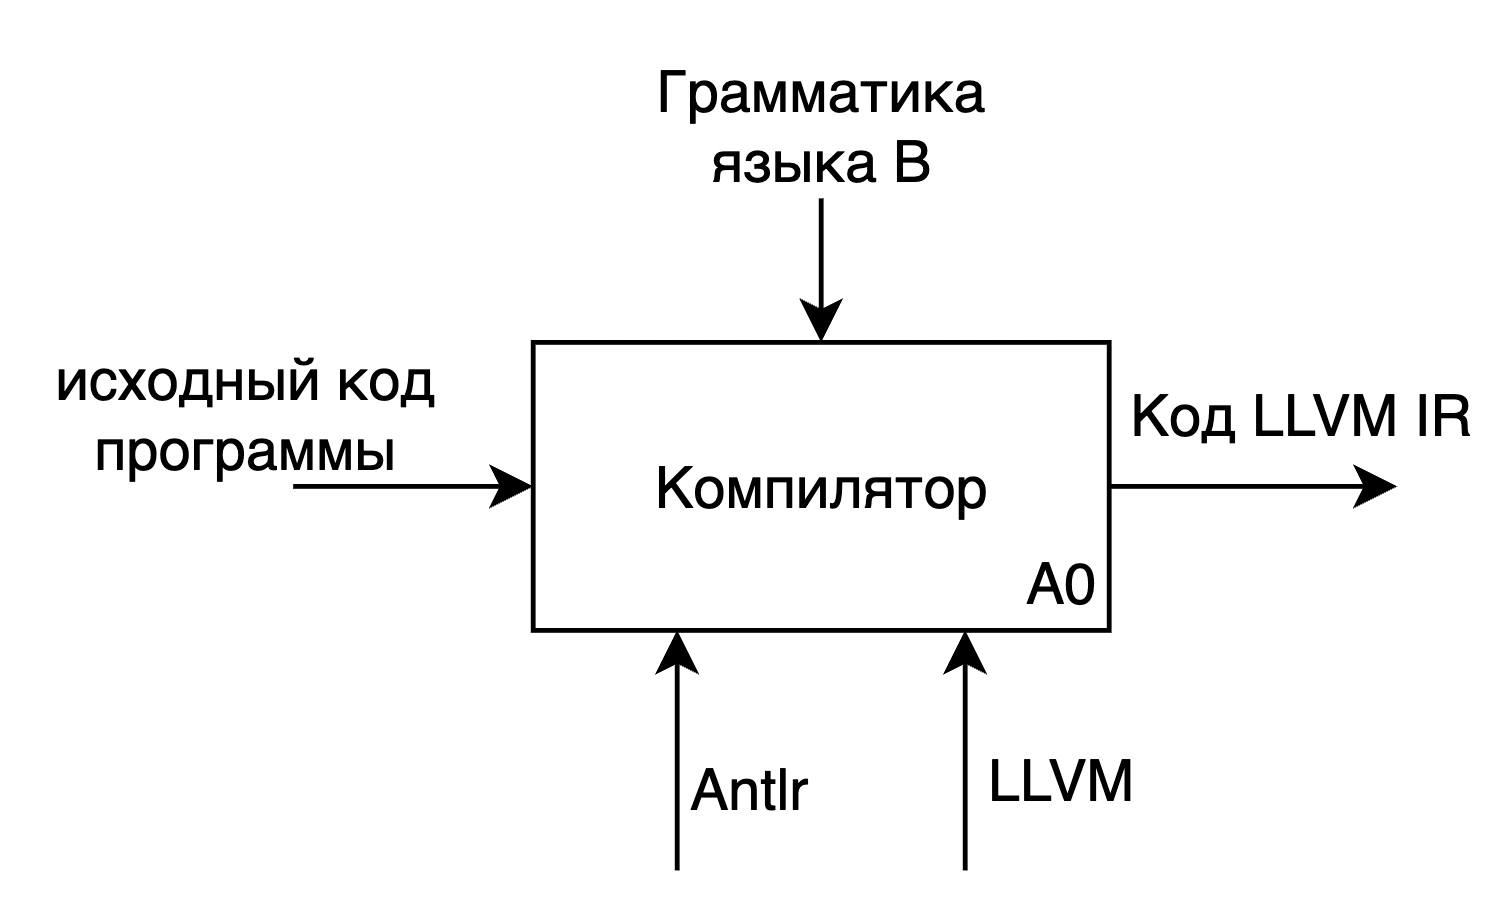
\includegraphics[scale = 0.2, angle=0]{../img/idef.jpg}}
		\caption{Концептуальная модель в нотации IDEF0}
		\label{fig:idef0-0}
	\end{center}
\end{figure}


На рисунке представлена детализированная концептуальная модель в нотации IDEF0.
ANTLR фронтенд получает на вход исходный код программы и генерирует конкретное синтаксическое дерево, на основе которого компилятором генерируется LLVM IR.

\begin{figure}[H]
	\begin{center}
		{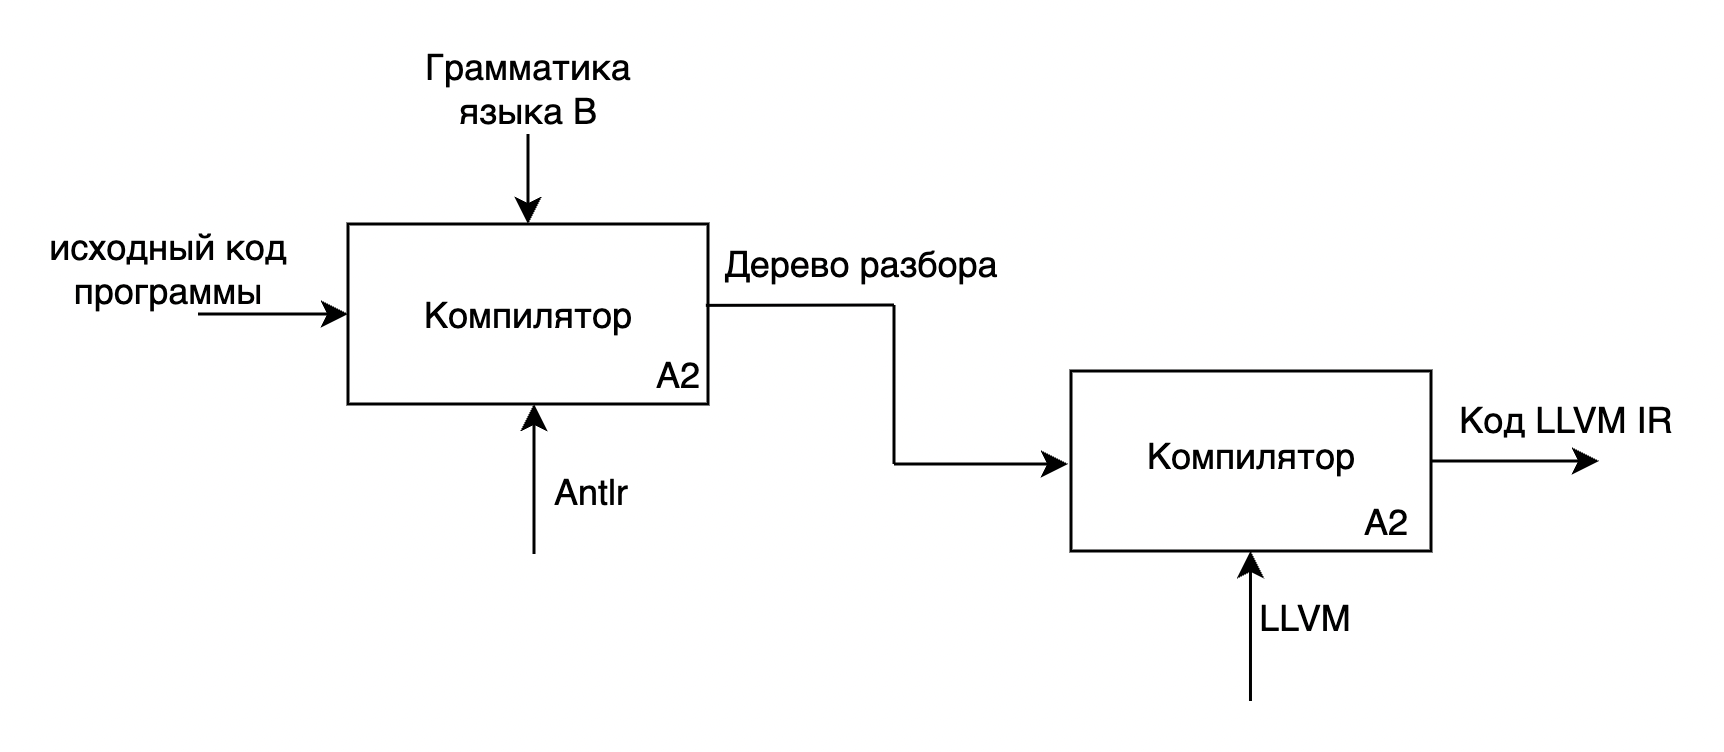
\includegraphics[scale = 0.3, angle=0]{../img/idef-detailed.jpg}}
		\caption{Детализированная концептуальная модель в нотации IDEF0}
		\label{fig:idef0-0}
	\end{center}
\end{figure}


\section{Язык программирования В}

Язык программирования B представляет собой упрощённый процедурный язык, исторически разработанный как предшественник языка C.
В языке B отсутствует поддержка структур, модульности или объектно-ориентированных конструкций, однако активно используются управляющие конструкции (циклы, условные операторы, переходы), поэтому компилятору необходимо эффективно обрабатывать вложенные блоки, jump-операции (включая goto) и переменные области видимости.
Основными особенностями языка являются:

\begin{enumerate}
	\item \textbf{Неявная типизация}

	Одной из ключевых особенностей языка программирования B, непосредственно влияющей на реализацию компилятора, является неявная типизация переменных при их объявлении. 
	В соответствии с грамматикой языка, переменные могут быть объявлены с использованием ключевого слова auto без указания типа и без инициализации, например: auto a;. 
	В этом случае тип переменной не фиксируется на момент объявления и остаётся неопределённым до момента первого присваивания, например: a = 5;. 
	Тип переменной выводится на основе правой части выражения присваивания, и именно тогда происходит выделение памяти с использованием подходящего LLVM-типа. 
	Для реализации такого поведения компилятор использует специальный механизм отслеживания неинициализированных переменных: все переменные, объявленные через auto без присваивания, помещаются во внутренний список. 
	При встрече с операцией присваивания компилятор проверяет, содержится ли имя переменной в этом списке. Если переменная обнаружена, осуществляется анализ типа правой части выражения, после чего переменной выделяется память соответствующего типа (например, i32 для целых значений) с помощью инструкции alloca, и она удаляется из списка неинициализированных. 
	Если же переменная уже была проинициализирована ранее, выполняется обычное присваивание. 
	Такой подход позволяет гибко и прозрачно реализовать ленивую типизацию переменных, сохраняя поведение языка и обеспечивая корректную генерацию промежуточного представления.

	\item \textbf{Отсуствие возвращаемого значения функции в ее сигнатуре}

	Ещё одной характерной особенностью языка B является отсутствие явно определяемого возвращаемого значения в сигнатуре функции. 
	В отличие от большинства современных языков программирования, таких как C, C++ или Java, где возвращаемый тип указывается до имени функции, язык B вовсе не предусматривает подобной конструкции на синтаксическом уровне. 
	Это решение значительно упрощает синтаксис и семантический анализ, избавляя компилятор от необходимости отслеживания типа результата и сопоставления его с выражением в операторе return. 
	Однако такая упрощённость накладывает и определённые ограничения: функции в языке B могут использоваться лишь как подпрограммы, выполняющие побочные действия (например, модификация переменных, вывод на экран и т. д.), но не как выражения, результат которых может быть использован в более широком контексте. 
	При реализации компилятора данная особенность позволяет отказаться от поддержки стека возвращаемых значений и существенно упростить логику генерации промежуточного представления, так как отсутствует необходимость управлять возвратом значения из функции через регистры или выделенную память. 
	С точки зрения концептуального дизайна, это сближает язык B с процедурными языками раннего поколения и подчёркивает его ориентированность на обучение принципам трансляции, а не на построение полнофункционального языка общего назначения.

	\item \textbf{Поддержка только двух типов переменных: INT и STRING}

	Язык программирования B характеризуется минималистичной системой типов: он поддерживает лишь два основных типа переменных — целочисленный (INT) и строковый (STRING). 
	Такое упрощение типовой системы было заложено в грамматике языка и отражает его учебно-исследовательскую направленность. 
	Несмотря на кажущуюся ограниченность, это решение обладает важными импликациями для реализации компилятора. 
	Во-первых, упрощается процесс синтаксического и семантического анализа: отсутствует необходимость в реализации сложных правил приведения типов, проверок на совместимость и перегрузок операций. 
	Во-вторых, достаточно однозначно определяется поведение операций: арифметические и логические действия применимы только к значениям типа INT, тогда как строковые значения допускаются, например, только в контексте присваивания или вывода. 
	Тем не менее, ограниченный типовой ландшафт требует особого внимания при генерации промежуточного представления: компилятору необходимо чётко различать указатели на строки (часто реализуемые через CreateGlobalString в LLVM) и аллоцированные значения i32, обеспечивая при этом корректное размещение, обращение и копирование данных. 
	Такая строгость в типизации при минимальном числе доступных типов служит хорошей основой для освоения ключевых принципов компиляции без усложнения логики трансляции.
\end{enumerate}

Полная грамматика языка B представлена в приложении A.

\section{Метод обхода AST}

Для обхода абстрактного синтаксического дерева, построенного ANTLR, использовался паттерн посетитель (Visitor). 
ANTLR генерирует базовый класс BaseVisitor, в котором для каждого правила грамматики определён метод visit<RuleName>. 
Эти методы вызываются вручную при рекурсивном обходе дерева и могут быть переопределены для обработки конкретных узлов.

В отличие от слушателя, посетитель реализует явный контроль обхода: вызовы visit выполняются программно, что даёт большую гибкость при интерпретации или трансформации дерева. Это позволяет, например, изменять порядок обхода или реализовывать короткую обработку без посещения поддеревьев.

ANTLR генерирует интерфейс слушателя специфичный для заданной грамматики и содержащий exit- и enter-методы для каждого правила, которые нужно реализовать в зависимости от решаемой задачи.
На рисунках \ref{img:listener} и \ref{img:walker} представлен порядок обхода дерева средствами ANTLR и порядок вызовов коллбэк-методов класса слушателя.

\begin{figure}[H]
	\begin{center}
		{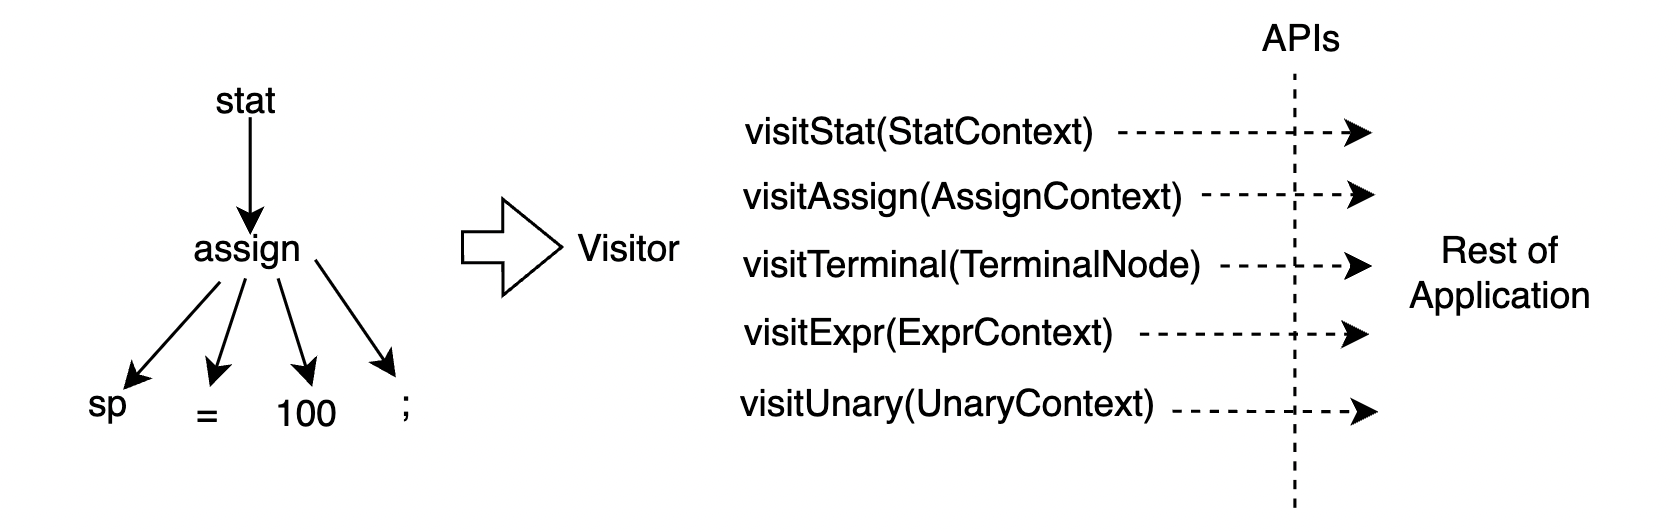
\includegraphics[scale = 0.3, angle=0]{../img/visitor.jpg}}
		\caption{Порядок обхода дерева разбора}
		\label{fig:idef0-0}
	\end{center}
\end{figure}

\begin{figure}[H]
	\begin{center}
		{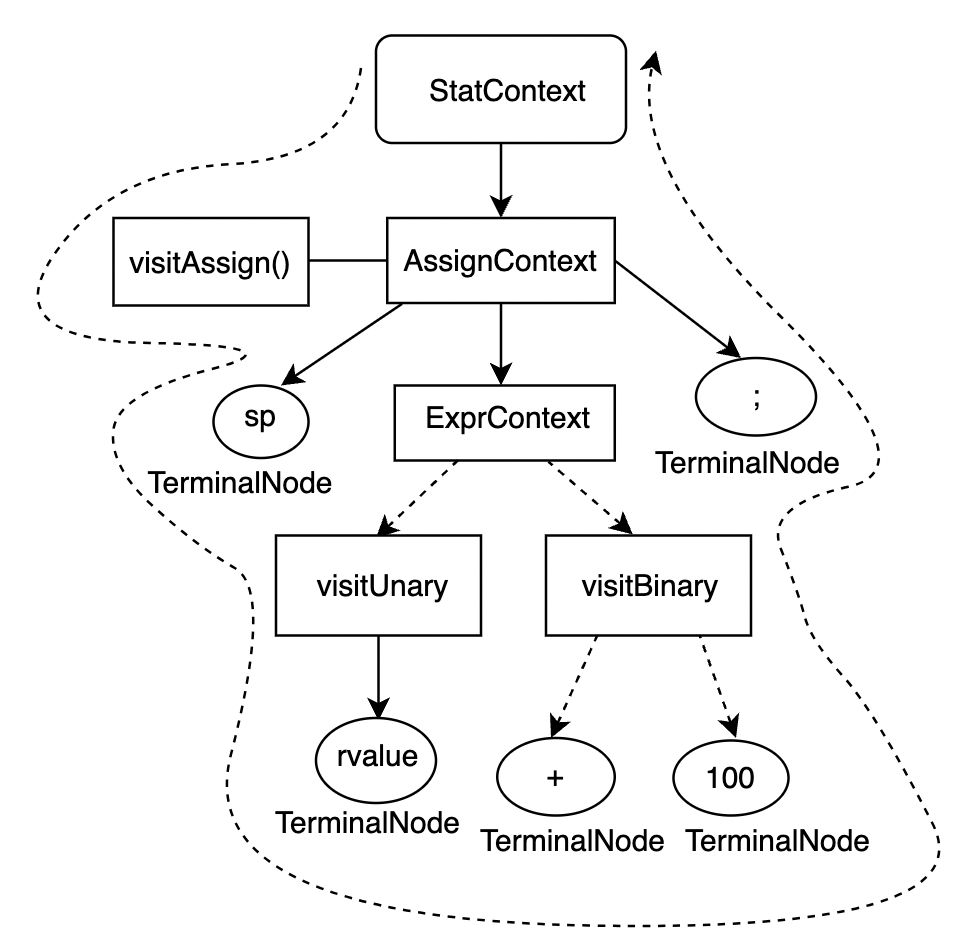
\includegraphics[scale = 0.3, angle=0]{../img/visitScheme.jpg}}
		\caption{Порядок вызова методов визитера}
		\label{fig:idef0-0}
	\end{center}
\end{figure}

\section{Генерация LLVM IR}

Для генерации кода LLVM IR необходимо произвести обход дерева разбора, полученного из парсера ANTLR, и в каждой вершине произвести генерацию соответствующую её типу.

Схема алгоритма для генерации кода LLVM IR для цикла for с выражениями, выполняющимися до входа в цикл и после выполнения тела цикла, приведена на рисунках 4 и 5.

\begin{figure}[h!]
	\begin{center}
		{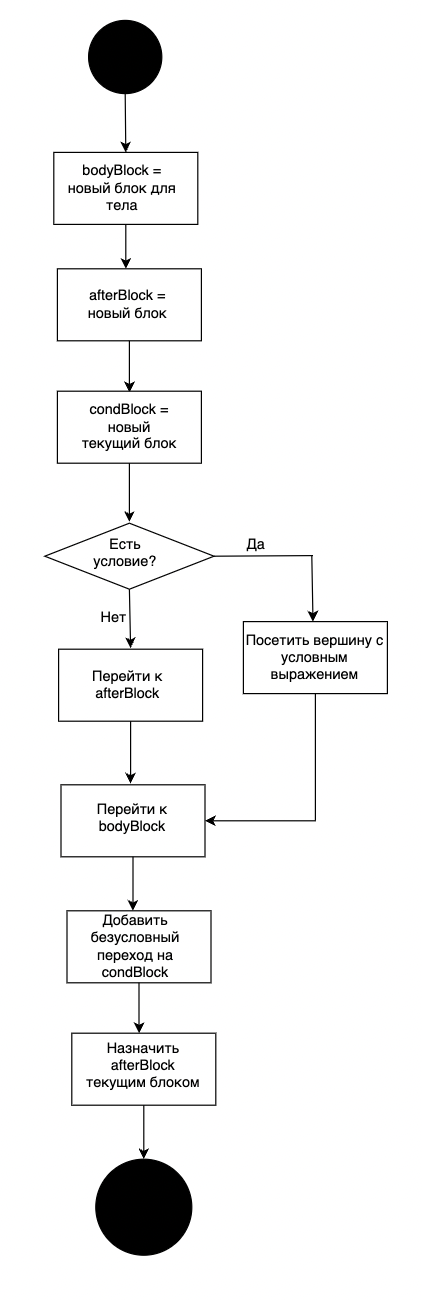
\includegraphics[scale = 0.5, angle=0]{../img/while_algo.jpg}}
		\caption{Схема генерации кода для тела и выражения, выполняющегося после тела цикла while}
		\label{fig:idef0-0}
	\end{center}
\end{figure}